\section{ИЗМЕРЕНИЕ УСКОРЕНИЯ}

\subsection{ИЗМЕРЕНИЕ ВРЕМЕНИ РАБОТЫ АЛГОРИТМА}

Для проверки закона Амдала необходимо определить ускорение алгоритма при различном числе процессов. Ускорение определяется на основе времени работы алгоритма. Время работы алгоритма оказывается зависящим от ширины блока $n_b$, выбор наиболее эффективного размера блока $n_b$ зависит от характеристик тестового стенда и составляет для рассматриваемой машины $n_b = 10$.

Время работы оптимизированной программы при различном числе потоков и различной вычислительной сложности (для $n=100,\, 1100,\, 2500,\, 5000,\, 10000$) мерилось с помощью bash-сценария, который представлен в Листинге \ref{listing:bash}. Для каждого $n$ измерения проводились по три раза. Стоит отметить, что внутри самой программы время мерилось с помощью функции \texttt{MPI\_WTIME}.
\begin{lstlisting}[language=bash, style=fortran, caption={Сценарий запуска численных экспериментов на языке bash.}, label={listing:bash}]
#!/bin/bash
# compiling the program
mpifort -O2 cholesky_mpi_block_test.f90 -o cholesky_mpi_block_test
# Entering the maximum number of processes, the amount of experiments and the block width
echo "Enter the maximum number of processes"
read max_nproc
echo "Enter the amount of experiments"
read nexp
echo "Enter the block width"
read nb
# Running the program in the following loop
for (( exp=1; exp<=$nexp; exp++ ))
do
   echo "Experiment: $exp"
   for (( nproc=1; nproc<=$max_nproc; nproc++ ))
   do
      echo "Number of processes: $nproc"
      filename=../data/$exp.$nproc.txt
      echo "# n; Execution time, sec" > $filename
      ns=(100 1100 2500 5000 10000)
      for n in ${ns[@]}
      do
         echo "n: $n"
         # keeping time data
         echo "$n $nb" | mpirun -np $nproc ./cholesky_mpi_block_test 
         >> $filename
      done
   done
done
\end{lstlisting}
Результаты измерений приведены в Таблице \ref{tab:2}. На Рис. \ref{fig:t_vs_threads} показана зависимость среднего времени выполнения оптимизированной версии программы от числа потоков при различной вычислительной сложности, вертикальными линиями отмечены плюс и минус одно стандартное отклонение (корень из дисперсии). 
\begin{figure}[htbp]
    \centering
    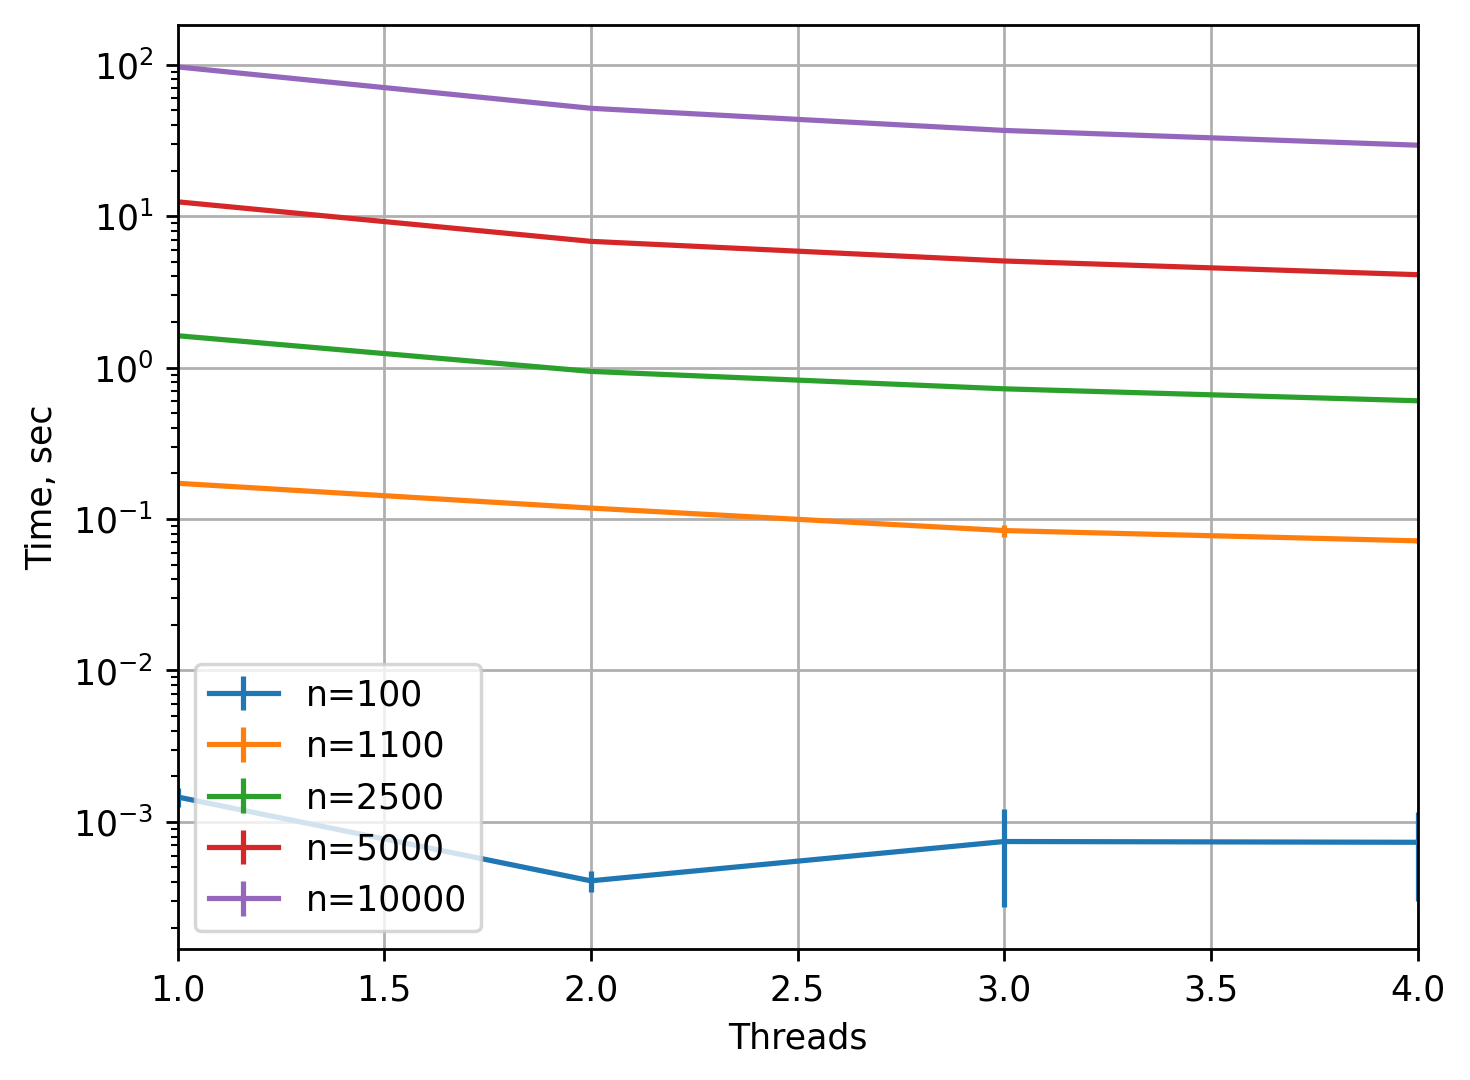
\includegraphics[scale=0.75]{fig/t_vs_threads.png}
    \caption{Время выполнения оптимизированной программы в секундах при различном числе потоков. Показано среднее за 3 эксперимента время. Вертикальными линиями отмечены плюс и минус одно стандартное отклонение (корень из дисперсии; они не всегда различимы из-за своей малости).}
    \label{fig:t_vs_threads}
\end{figure}

\subsection{ИЗМЕРЕНИЕ УСКОРЕНИЯ АЛГОРИТМА}

Чтобы определить ускорение, для каждого $n=100,\, 1100,\, 2500,\, 5000,\, 10000$ вычисляется среднее время работы алгоритма в последовательном режиме $t^{(n)}_1$ с абсолютной погрешностью $\Delta t^(n)_1$, которая равна стандартному отклонению времени работы алгоритма в последовательном режиме. Далее считается само ускорение алгоритма с матрицей размера $n\times n$ для $T$ потоков по формуле
\begin{equation}
    k^{(n)}_T = \dfrac{t^{(n)}_1}{t^{(n)}_T},
\end{equation}
где $t^{(n)}_T$ --- среднее время работы алгоритма с матрицей размера $n\times n$ на $T$ потоках. Погрешность ускорения рассчитывается следующим образом:
\begin{equation}
   \Delta k^{(n)}_T = \dfrac{\Delta t^{(n)}_1 \cdot t^{(n)}_T + \Delta t^{(n)}_T \cdot t^{(n)}_1}{(t^{(n)}_T)^2}.
\end{equation}

На Рис. \ref{fig:speedup_vs_threads} показана зависимость ускорения от числа потоков при различной вычислительной сложности, закрашенные области соответствуют плюс и минус одному стандартному отклонению.
\begin{figure}[htbp]
    \centering
    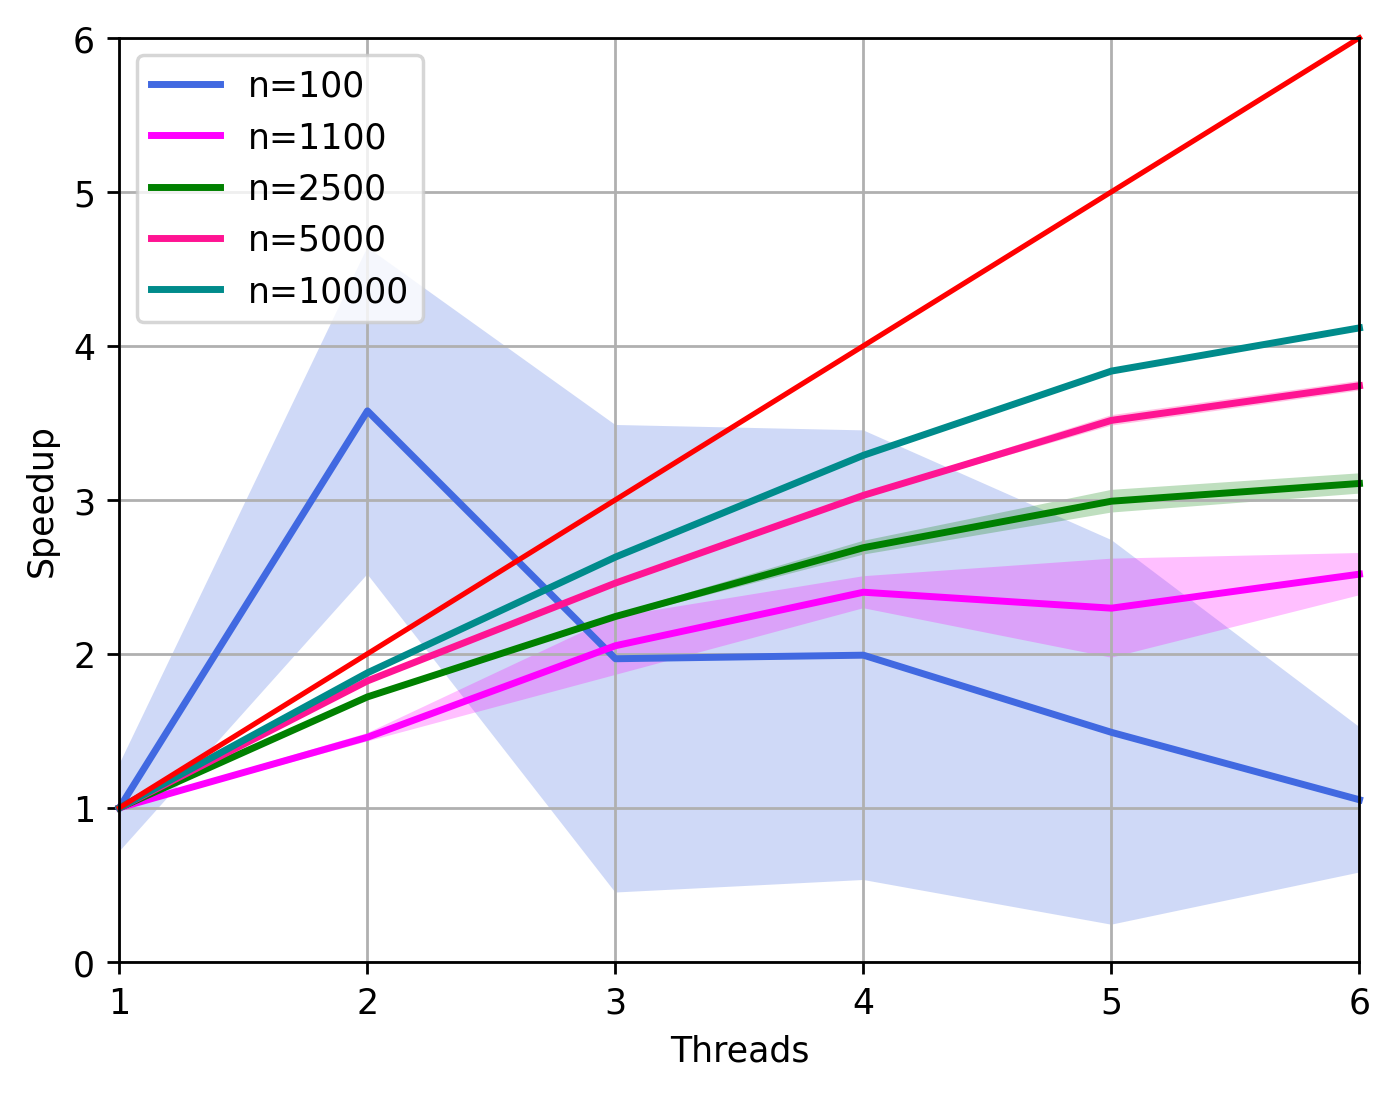
\includegraphics[scale=0.75]{fig/speedup_vs_threads.png}
    \caption{Ускорение оптимизированной программы при различном числе потоков, закрашенные области соответствуют плюс и минус одному стандартному отклонению (для некоторых линий закрашенных областей может быть не видно, это свидетельствует лишь о малости ошибки). Красная линия обозначает идеальный случай, когда ускорение равно числу потоков.}
    \label{fig:speedup_vs_threads}
\end{figure}
